\section{Sumas por filas y columnas}

Se tiene un archivo datos\_1.txt con números dispuestos de la siguiente forma. No necesariamente con la misma cantidad de filas y columnas.
\begin{figure}[h]
    \centering
    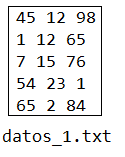
\includegraphics[scale=0.9]{Guia/datos.png}
\end{figure}
\begin{itemize}
    \item[a.] Cree la función \texttt{suma\_lineas(nombre\_archivo)} que retorne una lista con las sumas de las líneas del archivo.
    \item[b.] Desarrolle la función \texttt{suma\_columnas(nombre\_archivo)} que retorne una lista con las columnas del archivo.
\end{itemize}